The Server Side Application is the module that is responsible for producing a solution to a user request. The architecture and implementation details of the SSA are presented in section \ref{sec:api_architecture}. Each request processed by the SSA is defined by a set of parameters that specify the aimed trip, as will be described in section \ref{sec:api_protocol}. Producing a solution to a user request also involves the communication with third party API's, as to obtain the necessary flight data, which is handled by the Data Management System, described in section \ref{sec:dms_implementation}. The actual production of a solution is managed by the Optimization System, described in section \ref{sec:os_implementation}. 


% \begin{figure}[H]
%   \centering
%   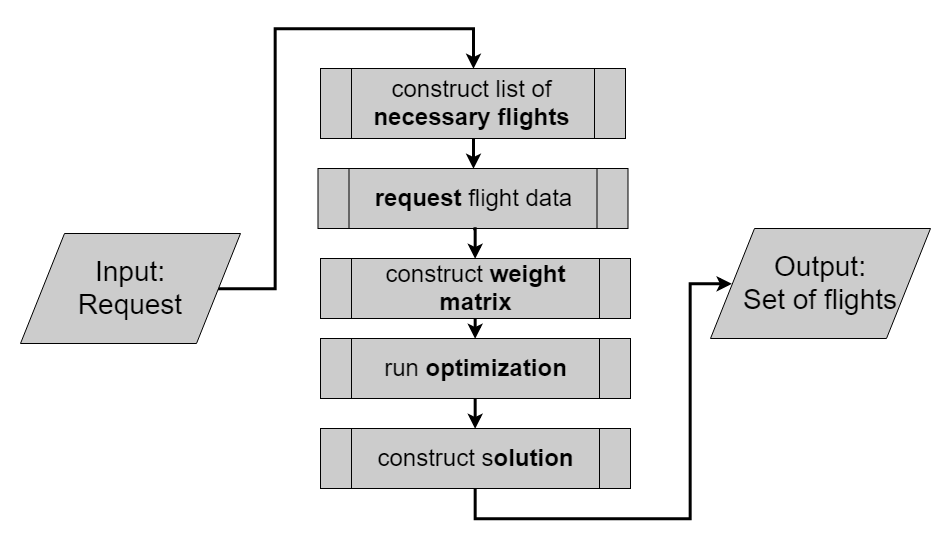
\includegraphics[width=\textwidth]{Figures/system_implementation/overall_flow_2.png}
%   \caption{Necessary steps to construct a solution to a user request.}
%   \label{fig:solution_steps}  
% \end{figure}